% !TEX program = lualatex
% Generated by new_lecture_note.sh
\documentclass[11pt]{article}

\usepackage{fontspec}
\usepackage{microtype}
\usepackage{mathtools,amssymb,amsfonts,amsthm,bm}
\usepackage{enumitem}
\usepackage{booktabs,array,xcolor}
\usepackage{tikz}
\usepackage{geometry,fancyhdr,setspace}
\usepackage[hidelinks]{hyperref}
\usepackage[nameinlink,noabbrev]{cleveref}

\geometry{margin=1in,headheight=15pt}
\setstretch{1.12}
\setlength{\parindent}{0pt}
\setlength{\parskip}{0.55em plus 0.12em minus 0.08em}
\setlength{\abovedisplayskip}{0.8em plus 0.2em minus 0.1em}
\setlength{\belowdisplayskip}{0.8em plus 0.2em minus 0.1em}
\allowdisplaybreaks[3]
\setlist{leftmargin=*,topsep=0.35em,itemsep=0.15em,parsep=0pt}

% ---------- Metadata ----------
\newcommand{\studentname}{Keshav Ramamurthy}
\newcommand{\coursename}{Math 118}
\newcommand{\courselongname}{Fourier Analysis}
\newcommand{\lecturenumber}{04}
\newcommand{\lecturetitle}{Lecture 04}
\newcommand{\lecturedate}{\today}

% ---------- Reusable notation ----------
\newcommand{\N}{\mathbb{N}}
\newcommand{\Z}{\mathbb{Z}}
\newcommand{\Q}{\mathbb{Q}}
\newcommand{\R}{\mathbb{R}}
\newcommand{\C}{\mathbb{C}}
\newcommand{\F}{\mathbb{F}}
\newcommand{\K}{\mathbb{K}}
\newcommand{\E}{\mathbb{E}}
\newcommand{\Prob}{\mathbb{P}}
\newcommand{\1}{\mathbf{1}}
\newcommand{\eps}{\varepsilon}
\newcommand{\dd}{\,\mathrm{d}}
\newcommand{\abs}[1]{\left\lvert#1\right\rvert}
\newcommand{\norm}[1]{\left\lVert#1\right\rVert}
\newcommand{\ip}[2]{\left\langle#1,#2\right\rangle}
\newcommand{\set}[1]{\left\{#1\right\}}
\newcommand{\given}{\,\middle\vert\,}
\newcommand{\indep}{\perp\!\!\!\perp}
\newcommand{\lto}{\longrightarrow}
\newcommand{\deriv}[2]{\frac{\mathrm{d}#1}{\mathrm{d}#2}}
\newcommand{\pderiv}[2]{\frac{\partial#1}{\partial#2}}
\DeclareMathOperator{\Aut}{Aut}
\DeclareMathOperator{\Hom}{Hom}
\DeclareMathOperator{\Ker}{ker}
\DeclareMathOperator{\im}{im}
\DeclareMathOperator{\rank}{rank}
\DeclareMathOperator{\nullity}{nullity}
\DeclareMathOperator{\Span}{span}
\DeclareMathOperator{\Var}{Var}
\DeclareMathOperator{\Cov}{Cov}

% ---------- Note environments ----------
\newtheoremstyle{notestyle}{0.7em}{0.7em}{\itshape}{}{}{\bfseries}{.5em}{}
\theoremstyle{notestyle}
\newtheorem{theorem}{Theorem}[section]
\newtheorem{lemma}[theorem]{Lemma}
\newtheorem{proposition}[theorem]{Proposition}
\newtheorem{corollary}[theorem]{Corollary}
\theoremstyle{definition}
\newtheorem{definition}[theorem]{Definition}
\newtheorem{example}[theorem]{Example}
\newtheorem{remark}[theorem]{Remark}
\newenvironment{claim}{\par\noindent\textbf{Claim.}\ }{\par}
\newenvironment{idea}{\par\noindent\textit{Idea.}\ }{\par}
\newenvironment{proofsketch}{\par\noindent\textbf{Proof sketch.}\ }{\par}

% ---------- Header ----------
\pagestyle{fancy}
\fancyhf{}
\fancyhead[L]{\coursename}
\fancyhead[C]{\lecturetitle}
\fancyhead[R]{\studentname}
\fancyfoot[C]{\thepage}

\title{\vspace{-1.5em}\textbf{\coursename\ -- \lecturetitle}}
\author{\studentname}
\date{\lecturedate}

\begin{document}
\maketitle

\section{Lecture 4}
Last time, if $e_1,e_2,\cdots,e_n$ is an orthonormal basis for $V_0\subseteq V$, the orthogonal projection $P:V\rightarrow V_0$ is given by
$$
P_u=\sum_{n=1}^{N}\langle u,e_n\rangle e_n.
$$

\begin{itemize}
    \item $P$ is linear.
    \item $\langle Pu,v\rangle=\langle u,Pv\rangle$.
    \item If $v_0\in V_0$, then $Pv_0=v_0$.
    \item If $u\in V$ and $v\in V_0$, then $\langle u-Pu,v\rangle=0$.
\end{itemize}

\textbf{Theorem:}
$$
\langle u-u_0,v\rangle=0,\ \forall v\in V_0
\iff
\|u-u_0\|=\min_{v_0\in V_0}\|u-v_0\|.
$$

\[
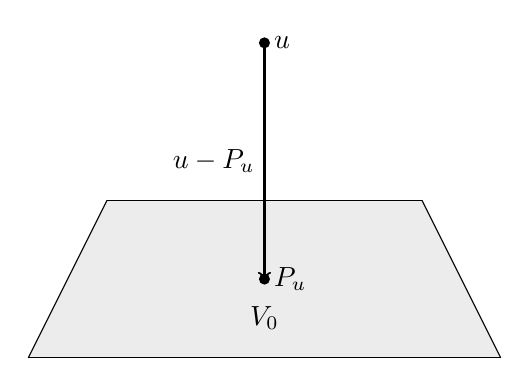
\begin{tikzpicture}
    % Plane
    \fill[gray!15] (-3,-1) -- (3,-1) -- (2,1) -- (-2,1) -- cycle;
    \draw (-3,-1) -- (3,-1);
    \draw (3,-1) -- (2,1);
    \draw (2,1) -- (-2,1);
    \draw (-2,1) -- (-3,-1);

    % Perpendicular vector
    \draw[->, thick] (0,3) -- (0,0);

    % Points
    \fill (0,3) circle (2pt) node[right] {$u$};
    \fill (0,0) circle (2pt) node[right] {$P_u$};

    % Labels
    \node at (0,-0.5) {$V_0$};
    \node[left] at (0,1.5) {$u-P_u$};
\end{tikzpicture}
\]

\textbf{Geometric Proof of Cauchy:} 
We prove the contrapositive, $\neg A\implies\neg B$.

Suppose $v_0\in V_0$ and $u_0$ is the closest point to $u$ in $V_0$. Since $u_0,v_0\in V_0$, we have
$$
u_0-v_0\in V_0.
$$

Set
$$
v=u_0-v_0.
$$

Then, by the assumption,
$$
\langle u-u_0,v\rangle=0.
$$

Therefore,
$$
\langle u-u_0,u_0-v_0\rangle=0.
$$

This gives the orthogonality condition in the theorem, and hence
$$
\langle u-u_0,v\rangle=0,\ \forall v\in V_0
\iff
\|u-u_0\|=\min_{v_0\in V_0}\|u-v_0\|.
$$
Notice $V = V_0 \oplus V_0^{\perp}$
\section{Norm of operators}
Let $X, Y$ be normed vector spaces.
A linear operator $A : X \rightarrow Y$ is bounded is there is a constant $M$  such that
is the "operator norm" of $A$:
$$||A|| = \sup_{x\ne 0} \frac{||Ax||}{||x||} = \sup_{||x||=1}||Ax||$$
To show that $||A|| = M$, you should either:
\par \textbf{1: } Show that $||Ax|| \le M ||x||, \forall x \in X$
\par \textbf{2: } Show that either product an $x_0$ such that $||Ax_0|| = M||x_0||$ or
show that if $K < M$ then $\exists x_0 \ne 0$, such that $||Ax_0|| > K||x_0||$
% \section{Definitions and notation}
%
\begin{definition}[First definition]
Write the definition and one sentence explaining why it matters.
\end{definition}

\section{Claims, theorems, and proof sketches}
\begin{claim}
State the claim in one precise sentence.
\end{claim}

\begin{proofsketch}
Record the key idea, the first useful equation, and the step that still needs checking.
\end{proofsketch}

\section{Examples and calculations}
\begin{example}[Lecture example]
Write the setup, the calculation, and the conclusion.
\end{example}

\section{Questions and follow-up}
\begin{itemize}
  \item What is still unclear?
  \item Which exercise or reading should I revisit?
  \item TODO:
\end{itemize}

\end{document}
